\documentclass[10pt,twocolumn,letterpaper]{article}
\usepackage[a4paper, total={18cm, 26cm}]{geometry}
\usepackage{graphicx}
\usepackage{amsmath}
\usepackage{amssymb}
\usepackage{booktabs}
\usepackage{nicefrac}
\usepackage{algorithm}
\usepackage[algo2e]{algorithm2e} 
\usepackage{multirow}
\usepackage[pagebackref,breaklinks,colorlinks=true,linkcolor=blue]{hyperref}
\usepackage{indentfirst}

% Support for easy cross-referencing
\usepackage[capitalize]{cleveref}
\crefname{section}{Sec.}{Secs.}
\Crefname{section}{Section}{Sections}
\Crefname{table}{Table}{Tables}
\crefname{table}{Tab.}{Tabs.}

\begin{document}
\nocite{*}

\title{Examen : Doc N°2}
\author{GIRARDOT Axel}
\maketitle

%% Here goes your code

\begin{figure*}
    \centering
    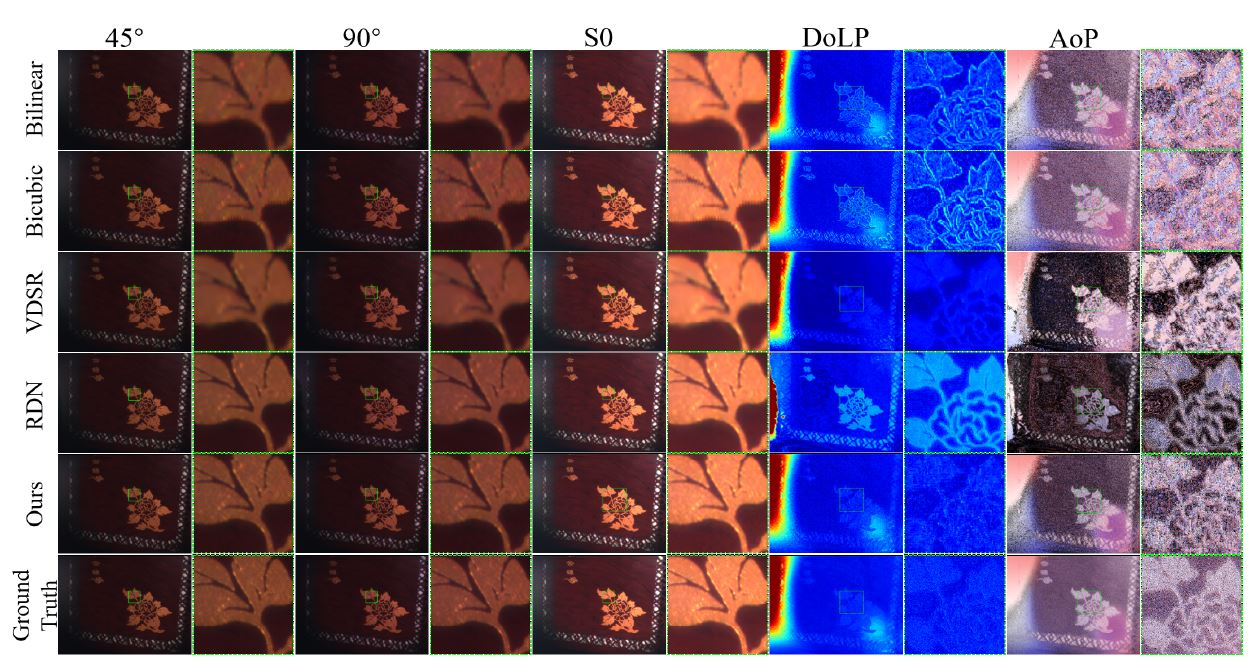
\includegraphics[width=15cm]{Image/image_fig5.JPG}
    \caption{We randomly choose a scene for a sample of visual comparison. Reconstruction results of 45◦, 90◦, S0, DoLP, and AoP by Bilinear, Bicubic, RDN and our proposed method. Zooming in will show more details.}
    \label{fig:5}
\end{figure*}


\begin{table}[H]
    \centering
    \begin{tabular}{c|lccccccc}
        \hline \hline
        \hline
        Method & PSNR  & SSIM & CA & S0 & DoLP & AoP & Time Consuming \\
        \hline
        {Zhang \cite{50_opticsletters}} & 35.241 & 0.903 & 23.063 & 33.620 & 14.320 & 10.234 & 296.95\\
        {Ours}& 36.786 & 0.950 & 23.788 & 33.272 & 14.900 & 10.462 & \textbf{8.4385}\\
        \hline
        \hline \hline
    \end{tabular}
    \caption{The results of comparisons with Zhang \cite{50_opticsletters}’s method. It should be noted that the size of test images is 200 × 200}
    \label{tab:table2}
\end{table}

\noindent requires a lot of calculations. Therefore, there is literally a limit on the size of the target image. In our case, the resolution of the input image is 1456 × 1088 which can not be processed by the maximum array size. For a fair comparison, we cut the test images to 200 × 200. As shown in table \ref{tab:table2}, the method proposed by Zhang \cite{50_opticsletters} can perform well in all evaluation metrics. However, the time consuming of Zhang \cite{50_opticsletters} is very large and cannot be ignored. The visualization of comparisons can be found in Fig. 5, from which we can perceive that the proposed method outperforms all other algorithms.

\subsection{Controlled Experiments}

\textbf{Regularization Parameter}. As shown in Tab. \cref{tab:table3}, the L1 norm regularization parameter will affect the performance of our proposed method. When the value of the L1 norm regularization parameter is 0.001, we can get better results.

\textbf{Different Dictionary}. Constructing appropriate dictionaries plays an important role in sparse representations and low-level vision task. A simple option would take the entire input date as the dictionary \cite{37_ICLM}. However, such a large dictionary is computationally expensive and consumes too much storage space. In addition, the large dictionary ignores details of polarimetric and chromatic information in this ill-posed problem. As we mentioned before, we also train twelve dictionaries based on each channel of the RGBPolarization data. Since there is no correlation between them during the demosaicing process, the reconstruction results are even worse. The results in Tab. \cref{tab:table3} verify our theory.

\begin{table}[H]
    \centering
    \begin{tabular}{l|cccccc}
        \hline
        Method & PSNR  & SSIM & CA & S0 & DoLP & AoP \\
        \hline
        {1-Dic} & 32.057 & 0.906 & 21.881 & 29.799 & 17.824 & 8.505\\
        {12-Dic}& 30.758 & 0.879 & 21.103 & 27.862 & 10.756 & 4.468 \\
        {$\lambda = 0.1$} & 31.579 & 0.933 & 23.113 & 29.810 & 19.783 & 10.730\\
        {$\lambda = 0.01$} & 32.426 & 0.938 & 22.973 & 31.219 & 20.570 & 10.252\\
        {$\lambda = 0.001$} & \textbf{35.078} & \textbf{0.943} & \textbf{23.473} & \textbf{31.833} & \textbf{22.777} & \textbf{11.152}\\
        \hline
    \end{tabular}
    \caption{The results of coontrolled experiments}
    \label{tab:table3}
\end{table}

\begin{figure}[H]
    \centering
    \begin{tabular}{ccc}
         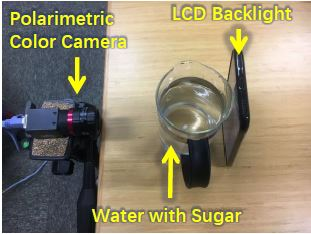
\includegraphics[width=4cm]{Image/imgA} &  
         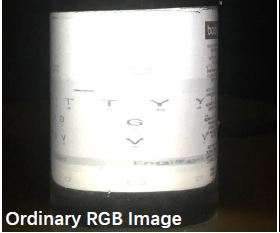
\includegraphics[width=4cm]{Image/imgB} & 
         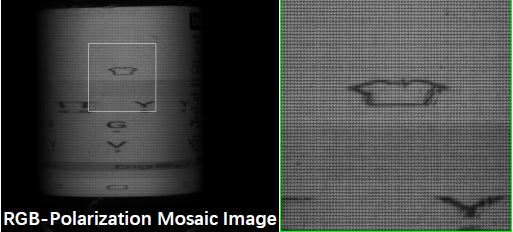
\includegraphics[width=4cm]{Image/imgC} 
         \\ (a) & (b) & (c) \\
         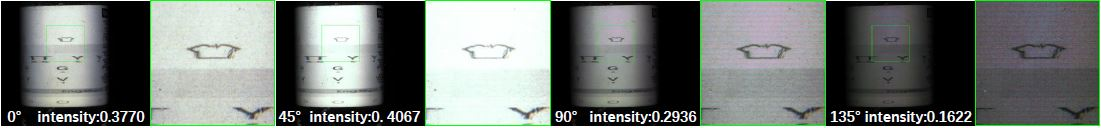
\includegraphics[width=10cm]{Image/imgD}
         \\  & (d) & \\
    \end{tabular}
    \caption{Application: (a) Application experiment setup; (b) An image of a glass of water with sugar recorded by a normal RGB camera; (c) An mosaic image of the same scene recorded by a polarimetric RGB camera(Lucid PHX050S-QC); (d) Four full-resolution RGBPolarization images reconstruct by our method.}
    \label{fig:Application}
\end{figure}

\subsection{Real Image}
\textbf{Application}. We conducted an application experiment to show the importance and effectiveness of joint color and
polarization demosaicing. Industrially, the method of measuring the concentration of sugar in a solution is to observe how the sugar affects the polarization of the light. Although measuring the concentration of sugar requires not only the
effect of the solution under polarized light but also many rigorous calibrations. Yet, observing the polarization declination is indeed one of the key steps in our joint demosaicing approach.

The traditional operation of rotating the polarizer not only causes deviation but also makes the experiment process
cumbersome. As shown in Fig. \ref{fig:Application}, the ordinary RGB image taken with a normal camera can not display the color of polarized light that passes through a sugar solution. On the contrary, instead of shifting the polarization angle, the polarized color camera can directly capture the RGBPolarization mosaic image by one snapshot. After processing along with the RGB-Polarization mosaic image by the proposed method, we can obtain \textbf{four polarization images with RGB information}. The ratio of the different value (calculated by RGB images) of known polarization angles (0◦, 45◦, 90◦, and 135◦) can help to calculate the concentration of sugar.

\textbf{Real Scene}. Polarimetric imagery can show the particular direction of the oscillation of the electric field described by the light. However, the ordinary RGB image taken with a normal camera can not display the color of polarized light. After the process of joint chromatic and polarimetric demosaicing, we can directly observe the color of the light in
different angles of polarization orientation. In this condition, we have captured images of a plastic box and a ruler in front of an LCD monitor. In addition, we also capture an image of the scene that the light of the screen passes through a plastic box. As shown in Fig. \ref{fig:7}, the reconstruction results show the color of the differently polarized light with good quality. This further verifies that our proposed methods can handle joint demosaicing of real scenes.

\begin{figure}
    \centering
    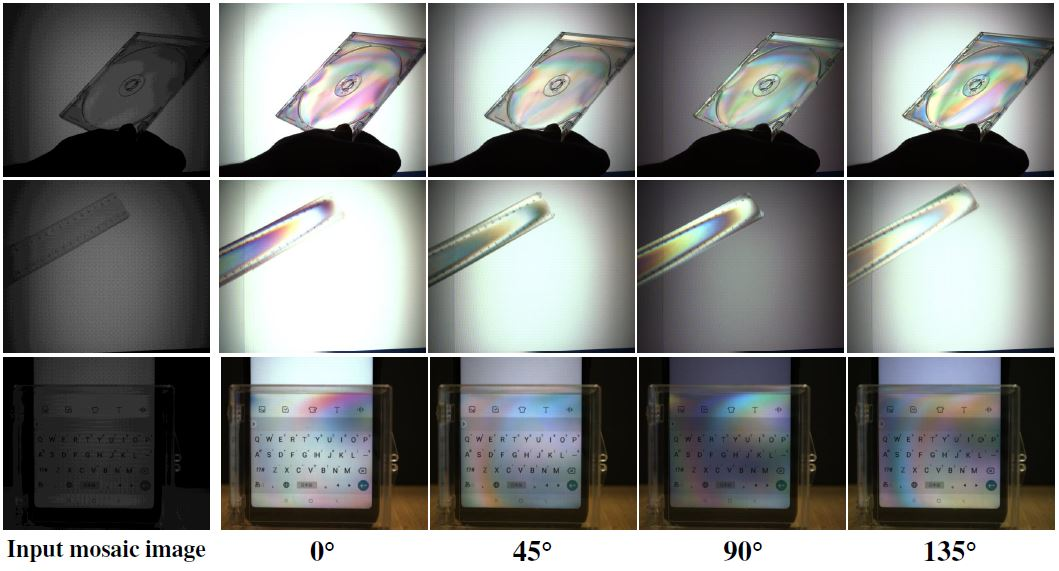
\includegraphics[width=8cm]{Image/image_fig7.JPG}
    \caption{Experiment results in the real scene.}
    \label{fig:7}
\end{figure}

\section{Conclusion}
In this paper, we first introduce joint chromatic and polarimetric demosaicing into the computer vision community. We build an RGB-Polarization data acquisition system by using a prism-based three-CMOS RGB camera and a motorized linear polarizer. As a very initial attempt, we propose a sparse representation-based demosaicing method by

{\small
\bibliographystyle{IEEEtran}
\bibliography{references}
}

\end{document}

